% ==========================================
% SECTION 4: TESTING & SIMULATION
% ==========================================
\section{Chiến Lược Kiểm Thử (Testing)}

% ------------------------------------------
% SLIDE: TỔNG QUAN CHIẾN LƯỢC KIỂM THỬ
% ------------------------------------------
\subsection{Mô hình phân tầng kiểm thử}
\begin{frame}{Chiến Lược Kiểm Thử Hệ Thống}
    Hệ thống được kiểm thử theo mô hình \textbf{kim tự tháp (V-model)}, đi từ khối đơn vị cô lập đến tích hợp toàn hệ thống 8 lõi:
    \vspace{0.2cm}

    \centering
    \begin{tikzpicture}[
        tier/.style={draw, thick, rounded corners, minimum height=0.7cm, font=\scriptsize\bfseries, align=center},
        arr/.style={->, >=stealth, thick, DeepBlue}
    ]
        \node[tier, fill=blue!8, minimum width=10cm] (t1) at (0, 0)
            {Tầng 1: Kiểm Thử Đơn Vị (Unit Testing) --- ALU, PC Logic, Pipeline Registers, Control Unit};
        \node[tier, fill=blue!15, minimum width=8cm] (t2) at (0, 1.0)
            {Tầng 2: Kiểm Thử Kết Nối (Interconnect \& Arbitration)};
        \node[tier, fill=blue!22, minimum width=6cm] (t3) at (0, 2.0)
            {Tầng 3: Kiểm Thử Tích Hợp Lõi Đơn (Single-Core)};
        \node[tier, fill=blue!30, minimum width=4cm] (t4) at (0, 3.0)
            {Tầng 4: Kiểm Thử Toàn Hệ Thống (8-Core)};

        \draw[arr] (t1) -- (t2);
        \draw[arr] (t2) -- (t3);
        \draw[arr] (t3) -- (t4);
    \end{tikzpicture}

    \vspace{0.3cm}
    \begin{columns}[T]
        \begin{column}{0.5\textwidth}
            \scriptsize
            \textbf{Công cụ sử dụng:}
            \begin{itemize}
                \item Biên dịch RTL: \texttt{Icarus Verilog (iverilog)}
                \item Chạy mô phỏng: \texttt{VVP}
                \item Trực quan Waveform: \texttt{GTKWave}
            \end{itemize}
        \end{column}
        \begin{column}{0.5\textwidth}
            \scriptsize
            \textbf{Tiêu chí Đạt/Hỏng (Pass/Fail):}
            \begin{itemize}
                \item So sánh tự động giá trị thanh ghi và bộ nhớ với kỳ vọng.
                \item Kiểm tra các bộ đếm Pipeline (\texttt{retired}, \texttt{stall}, \texttt{flush}).
                \item Đảm bảo không Deadlock, không Starvation.
            \end{itemize}
        \end{column}
    \end{columns}
\end{frame}

% ==========================================
% TẦNG 1: KIỂM THỬ ĐƠN VỊ (UNIT TESTING)
% ==========================================
\subsection{Tầng 1: Kiểm Thử Đơn Vị}

% --- SLIDE: Bảng tổng quan Unit Test ---
\begin{frame}{Tầng 1: Kiểm Thử Đơn Vị (Unit Testing)}
    Cô lập từng module cốt lõi để kiểm chứng tính đúng đắn của logic tổ hợp và tuần tự \textbf{trước khi ghép nối}:
    \vspace{0.15cm}

    \begin{table}[]
        \centering
        \scriptsize
        \begin{tabular}{llll}
            \toprule
            \textbf{Module} & \textbf{Testbench} & \textbf{Mục tiêu xác thực} & \textbf{Kết quả} \\
            \midrule
            Khối ALU & \texttt{alu\_tb.v} & 9 kịch bản: ADD, SUB, AND, OR, XOR, SLL, SRL, SLT, cờ Zero & \textcolor{green!60!black}{\textbf{PASS}} \\
            PC Logic & \texttt{pc\_logic\_tb.v} & Tăng tuần tự, nhảy Branch/Jump, giữ PC khi stall & \textcolor{green!60!black}{\textbf{PASS}} \\
            IF/ID Register & \texttt{tb\_if\_id.v} & Hold (đóng băng khi stall), Clear (flush NOP) & \textcolor{green!60!black}{\textbf{PASS}} \\
            ID/EX Register & \texttt{tb\_id\_ex.v} & Hold + Clear (chèn bubble NOP khi Load-Use) & \textcolor{green!60!black}{\textbf{PASS}} \\
            EX/MEM Register & \texttt{tb\_ex\_mem.v} & Hold (đóng băng khi Memory Stall) & \textcolor{green!60!black}{\textbf{PASS}} \\
            MEM/WB Register & \texttt{tb\_mem\_wb.v} & Hold đồng bộ, loại bỏ clear độc hại & \textcolor{green!60!black}{\textbf{PASS}} \\
            Control Unit & \texttt{tb\_control\_unit.v} & Giải mã đúng tín hiệu cho R/I/S/B/U/J-type & \textcolor{green!60!black}{\textbf{PASS}} \\
            Hazard Controller & \texttt{tb\_hazard\_controller.v} & Forwarding, Load-Use Stall, Branch Flush & \textcolor{green!60!black}{\textbf{PASS}} \\
            \bottomrule
        \end{tabular}
    \end{table}

    \vspace{0.1cm}
    \scriptsize
    Tổng cộng \textbf{8 module} được kiểm thử cô lập với kết quả \textbf{100\% PASS}. Kết quả Waveform chi tiết của từng module đã được trình bày ở phần Thiết kế.
\end{frame}

% ==========================================
% TẦNG 2: KIỂM THỬ KẾT NỐI (INTERCONNECT)
% ==========================================
\subsection{Tầng 2: Kiểm Thử Kết Nối}

% --- SLIDE: Interconnect Test Results ---
\begin{frame}[fragile]{Tầng 2: Kiểm Thử Kết Nối Bus \& Arbiter}
    Kiểm thử \textbf{Arbiter Round-Robin} + \textbf{Bus Controller} + \textbf{Data Memory} khi nhiều core cùng truy cập RAM chia sẻ.
    \vspace{0.1cm}

    \begin{columns}[T]
        \begin{column}{0.42\textwidth}
            \textbf{3 kịch bản kiểm thử:}
            \begin{enumerate}
                \scriptsize
                \item \textbf{Round-Robin Write/Read:} 4 core lần lượt ghi dữ liệu vào các địa chỉ khác nhau, sau đó đọc và xác thực.
                \item \textbf{LR/SC Atomic:} Core 0 thực hiện \texttt{LR} $\rightarrow$ \texttt{SC} thành công; sau đó \texttt{LR} $\rightarrow$ Core 1 ghi xen ngang $\rightarrow$ \texttt{SC} thất bại đúng kỳ vọng.
                \item \textbf{AMO Atomic Add:} \texttt{AMOADD +42} rồi \texttt{AMOADD +58} $\rightarrow$ tổng cuối = 100.
            \end{enumerate}
        \end{column}

        \begin{column}{0.58\textwidth}
            \begin{block}{Kết quả (\texttt{interconnect\_tb.v})}
                \fontsize{5.5pt}{6.5pt}\selectfont
                \begin{verbatim}
========================================
  TEST 1: Round-Robin Write/Read
========================================
  [PASS] C0: 0xaaaa0000
  [PASS] C1: 0xbbbb0001
  [PASS] C2: 0xcccc0002
  [PASS] C3: 0xdddd0003

========================================
  TEST 2: LR/SC Atomic Operations
========================================
  [PASS] SC SUCCESS
  [PASS] Mem=200
  [PASS] SC FAILED (expected)
  [PASS] Mem=999

========================================
  TEST 3: AMO Atomic Add
========================================
  AMOADD +42: old=0
  [PASS] Mem=42
  AMOADD +58: old=42
  [PASS] Mem=100

==========================================
  SUMMARY: 10 PASSED, 0 FAILED
==========================================
                \end{verbatim}
            \end{block}
        \end{column}
    \end{columns}
\end{frame}

% ==========================================
% TẦNG 3: KIỂM THỬ TÍCH HỢP LÕI ĐƠN
% ==========================================
\subsection{Tầng 3: Kiểm Thử Tích Hợp Lõi Đơn}

% --- SLIDE: Core Test Console Results ---
\begin{frame}[fragile]{Tầng 3: Kết Quả Kiểm Thử Lõi Đơn (Single-Core)}
    Tích hợp lõi \texttt{risc\_core.v} + \texttt{instr\_mem} + \texttt{data\_mem}. Nạp chương trình Assembly kiểm thử các phép toán, truy cập bộ nhớ và rẽ nhánh.
    \vspace{0.1cm}

    \begin{columns}[T]
        \begin{column}{0.48\textwidth}
            \textbf{Chương trình kiểm thử:}
            \begin{itemize}
                \scriptsize
                \item \texttt{ADDI x1, x0, 10} $\rightarrow$ x1 = 10
                \item \texttt{ADDI x2, x0, 20} $\rightarrow$ x2 = 20
                \item \texttt{ADD x3, x1, x2} $\rightarrow$ x3 = 30
                \item \texttt{SW x3, 0(x0)} $\rightarrow$ mem[0] = 30
                \item \texttt{LW x4, 0(x0)} $\rightarrow$ x4 = 30
                \item \texttt{BEQ x3, x4, +4} $\rightarrow$ branch taken
                \item \texttt{ADDI x5, x0, 1} $\rightarrow$ x5 = 1 (PASS)
            \end{itemize}
            \vspace{0.1cm}
            \begin{block}{Bằng chứng Pipeline hoạt động}
                \scriptsize
                \begin{itemize}
                    \item \texttt{retired = 67}: 67 lệnh hoàn thành commit.
                    \item \texttt{load\_use\_stall = 1}: Phát hiện 1 xung đột đọc-sau-nạp.
                    \item \texttt{flush = 62}: Xóa 62 lệnh rẽ nhánh sai hướng.
                \end{itemize}
            \end{block}
        \end{column}

        \begin{column}{0.52\textwidth}
            \begin{block}{Kết quả Console (\texttt{core\_tb.v})}
                \fontsize{5.5pt}{6.5pt}\selectfont
                \begin{verbatim}
=========================================
  CORE TEST RESULTS (after 200 cycles)
=========================================
  x1 (expect 10) = 10
    [PASS]
  x2 (expect 20) = 20
    [PASS]
  x3 (expect 30) = 30
    [PASS]
  x4 (expect 30) = 30
    [PASS]
  x5 (expect 1)  = 1
    [PASS] BRANCH worked!
  mem[0] (expect 30) = 30
    [PASS]

=========================================
  PIPELINE EVIDENCE
=========================================
  retired=67 mem_stall=4
  load_use_stall=1 flush=62
    [PASS] Pipeline counters show activity.

==========================================
  SUMMARY: 7 PASSED, 0 FAILED
==========================================
                \end{verbatim}
            \end{block}
        \end{column}
    \end{columns}
\end{frame}

% --- SLIDE: Waveform Lõi Đơn (Placeholder cho ảnh chụp) ---
\begin{frame}{Tầng 3: Waveform Mô Phỏng Lõi Đơn}
    \begin{block}{Giản đồ sóng Pipeline lõi đơn (\texttt{core\_tb.vcd})}
        \centering
        \vspace{0.3cm}
        % === BẠN CHỤP WAVEFORM VÀ THAY TÊN FILE TẠI ĐÂY ===
        \IfFileExists{design/test/risc_core.png}{%
            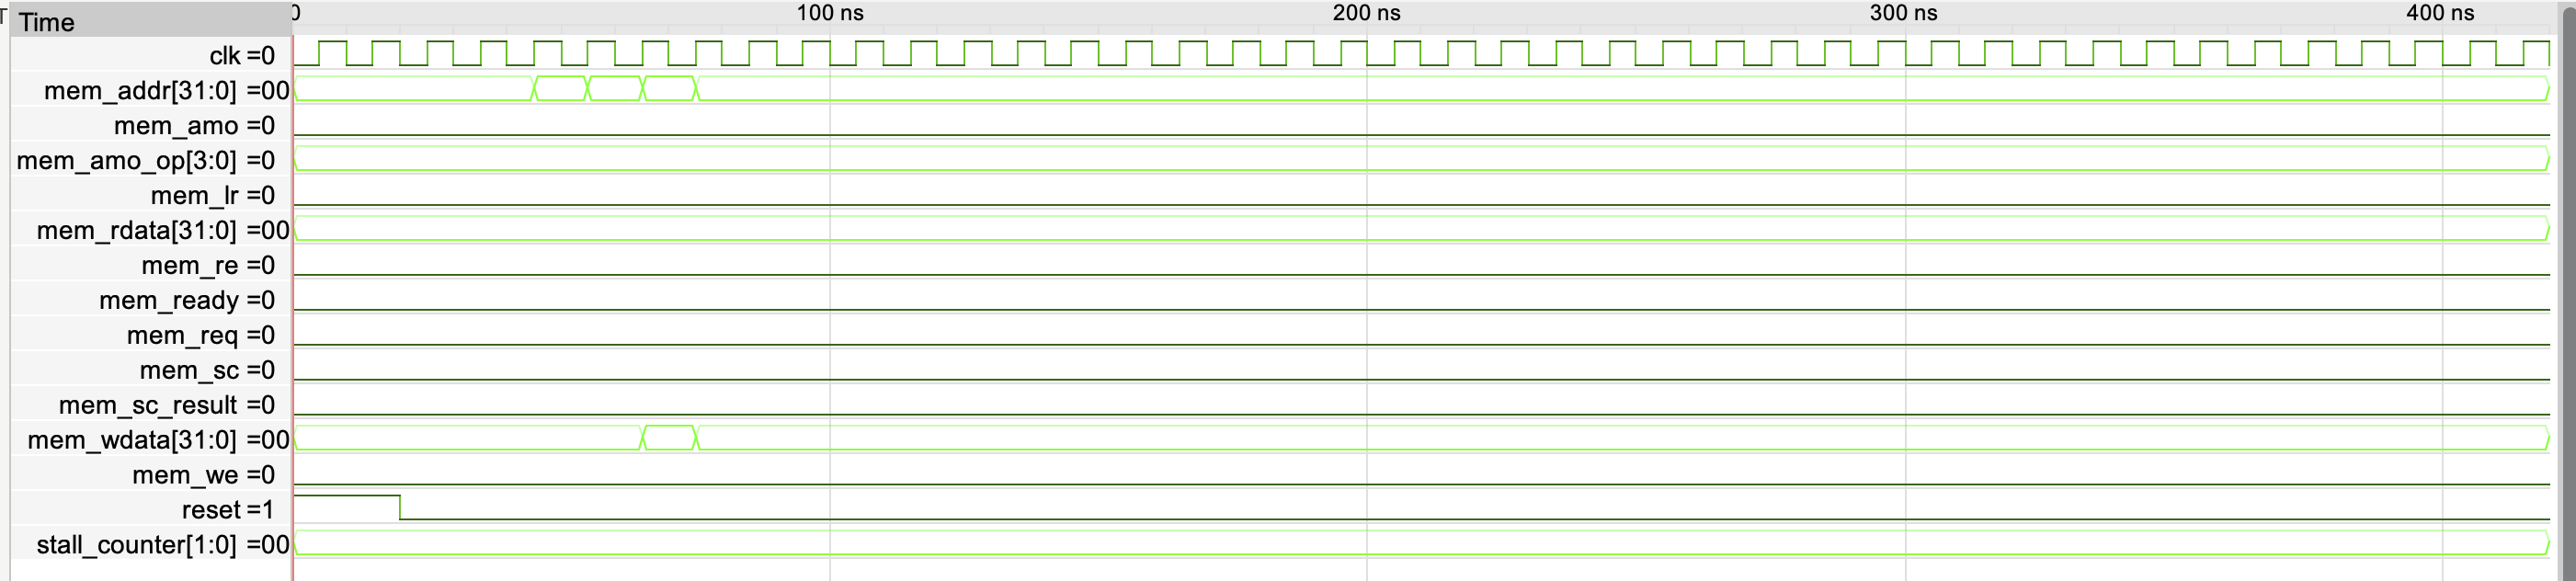
\includegraphics[width=0.92\textwidth]{design/test/risc_core.png}%
        }{%
            \fbox{\parbox[c][3.2cm][c]{0.88\textwidth}{\centering
                Chưa có ảnh \texttt{design/test/risc\_core.png}.}}
        }
        \vspace{0.3cm}
    \end{block}
    \vspace{0.1cm}
    \scriptsize
    \textbf{Phân tích Waveform:}
    \begin{itemize}
        \item Tín hiệu \texttt{PC} tăng tiến tuần tự +4 mỗi chu kỳ, nhảy đúng khi gặp lệnh \texttt{BEQ}/\texttt{JAL}.
        \item Các tín hiệu valid của pipeline (\texttt{if\_id\_valid}, \texttt{id\_ex\_valid}) bị xóa sạch tại thời điểm Flush.
        \item Tín hiệu \texttt{mem\_req} dựng lên khi core thực hiện \texttt{LW}/\texttt{SW}, \texttt{mem\_ready} phản hồi sau 1 chu kỳ.
    \end{itemize}
\end{frame}

% ==========================================
% TẦNG 4: KIỂM THỬ TOÀN HỆ THỐNG 8-CORE
% ==========================================
\subsection{Tầng 4: Kiểm Thử Toàn Hệ Thống}

% --- SLIDE: System Test Console Results ---
\begin{frame}[fragile]{Tầng 4: Kết Quả Kiểm Thử Hệ Thống 8-Core}
    Tích hợp toàn bộ 8 lõi CPU chạy song song, kết nối qua \textbf{Arbiter} và \textbf{Bus Controller} truy cập RAM dùng chung.
    \vspace{0.1cm}

    \begin{columns}[T]
        \begin{column}{0.42\textwidth}
            \textbf{Đánh giá hiệu năng:}
            \begin{itemize}
                \scriptsize
                \item 8 core cùng thực thi, ghi/đọc RAM dùng chung \textbf{không deadlock}.
                \item \texttt{grant} công bằng cho tất cả các nhân.
                \item \texttt{mem\_stall} tăng tuyến tính từ Core 0 $\rightarrow$ Core 7 $\Rightarrow$ đúng hành vi Round-Robin.
            \end{itemize}

            \begin{block}{Chỉ số xác thực}
                \scriptsize
                \begin{itemize}
                    \item \texttt{mem[0] == 42}: Dữ liệu ghi đúng.
                    \item \texttt{mem[1] == 99}: Marker hoàn thành.
                    \item 8/8 core: \texttt{grant > 0} và \texttt{retired > 0}.
                \end{itemize}
            \end{block}
        \end{column}

        \begin{column}{0.58\textwidth}
            \begin{block}{Kết quả Console (\texttt{system\_tb.v})}
                \fontsize{5pt}{6pt}\selectfont
                \begin{verbatim}
=========================================================
  BAT DAU MO PHONG HE THONG 8 LOI PIPELINE
=========================================================
  Kiem tra mem[0] (Ky vong: 42) = 42
    [PASS] Shared memory data dung.
  Kiem tra mem[1] addr 4 (Ky vong: 99) = 99
    [PASS] 8 core hoan thanh khong deadlock.

=========================================================
  PIPELINE / BUS EVIDENCE
=========================================================
  Core 0: grant=3 retired=163 mem_stall=13 flush=159
  Core 1: grant=3 retired=163 mem_stall=14 flush=159
  Core 2: grant=3 retired=163 mem_stall=15 flush=159
  Core 3: grant=3 retired=163 mem_stall=16 flush=159
  Core 4: grant=4 retired=161 mem_stall=17 flush=157
  Core 5: grant=4 retired=161 mem_stall=18 flush=157
  Core 6: grant=4 retired=161 mem_stall=19 flush=157
  Core 7: grant=4 retired=161 mem_stall=20 flush=157

  TONG KET: 10 PASSED, 0 FAILED
=========================================================
                \end{verbatim}
            \end{block}
        \end{column}
    \end{columns}
\end{frame}

% --- SLIDE: Waveform Hệ Thống 8-Core (Placeholder cho ảnh chụp) ---
\begin{frame}{Tầng 4: Waveform Mô Phỏng Hệ Thống 8-Core}
    \begin{block}{Giản đồ sóng toàn hệ thống (\texttt{system\_tb.vcd})}
        \centering
        \vspace{0.3cm}
        % === BẠN CHỤP WAVEFORM VÀ THAY TÊN FILE TẠI ĐÂY ===
        \IfFileExists{design/test/top_8core.png}{%
            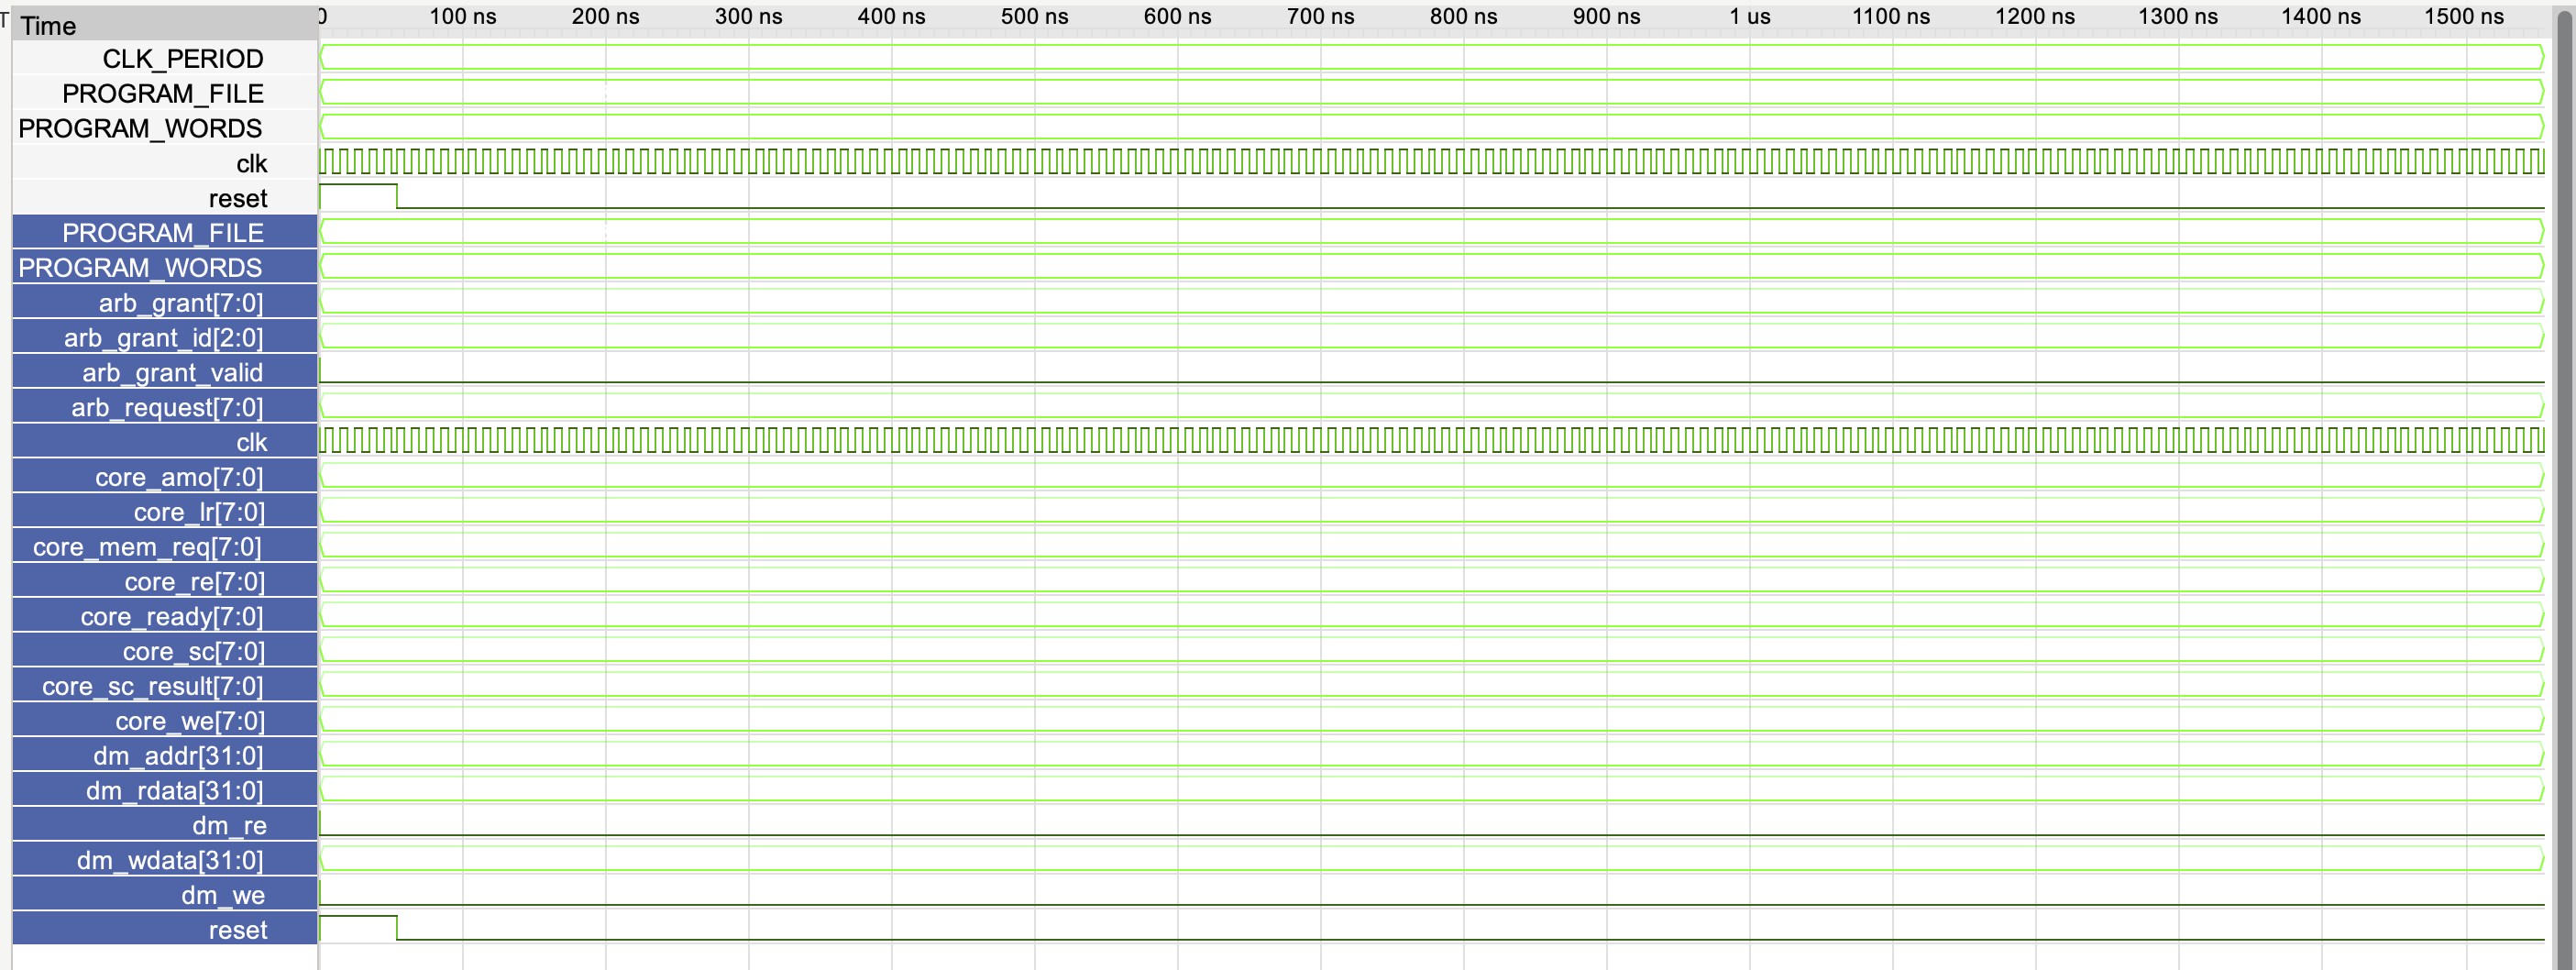
\includegraphics[width=0.92\textwidth]{design/test/top_8core.png}%
        }{%
            \fbox{\parbox[c][3.2cm][c]{0.88\textwidth}{\centering
                Chưa có ảnh \texttt{design/test/top\_8core.png}.}}
        }
        \vspace{0.3cm}
    \end{block}
    \vspace{0.1cm}
    \scriptsize
    \textbf{Phân tích Waveform:}
    \begin{itemize}
        \item Tín hiệu \texttt{grant[7:0]} của Arbiter phân phối quyền truy cập bus xoay vòng công bằng giữa 8 lõi.
        \item Các core chờ đợi (\texttt{mem\_stall}) khi chưa được cấp bus, tiếp tục xử lý Pipeline khi nhận \texttt{mem\_ready}.
        \item Không xảy ra tình trạng 2 core đồng thời giữ \texttt{grant = 1} (đảm bảo Mutual Exclusion).
    \end{itemize}
\end{frame}
